\documentclass{beamer}
%\usetheme{Berkeley}
% packages
\usepackage {lmodern}
\usepackage {graphicx}
\usepackage {caption}
\usepackage {gensymb}
\usepackage[LGRgreek]{mathastext}
\usepackage[T1]{fontenc}
\setbeamerfont{footnote}{size=\tiny}
\usepackage[backend=biber, autocite=superscript]{biblatex}

\graphicspath {{images/}}

%\setbeamertemplate{bibliography item}{}

\title{Venture}
\author{Group 1}
\institute{CS 329E \\ The Universty of Texas at Austin}
\date{March 26, 2017}

\begin{document}
\frame{\titlepage}

\section{Group Members}
\begin{frame}
\frametitle{Group Members}
    \begin{itemize}
        \item Justin Chao
        \item Julianne Crea
        \item Connie Liu
    \end{itemize}
\end{frame}

\section{Application Description}
\begin{frame}
\frametitle{Application Description}
    \begin{itemize}
        \item trip-planning often involves just making a Word or Google doc and inserting links to
            other websites.
        \item Venture provides simple and convenient planning of trip itineraries 
        \item reinforces safe-spending-habits by actively tracking your expenses.
        \item increases efficiency in planning for travel to multiple places by putting it all in one app.
        \item provides for a more organized and therefore, more enjoyable travel experience.
    \end{itemize}
\end{frame}

\section{Target Audience}
\begin{frame}
\frametitle{Target Audience}
    \begin{itemize}
        \item Anyone who enjoys traveling and likes to have well-organized travel plans
    \end{itemize}
\end{frame}

\section{Application Functionality}
\begin{frame}
\frametitle{Application Functionality}
    \begin{itemize}
        \item Firebase backend with Google user authentication will be implemented.
        \item user options (user profile, themes)
		\item search for non-stop flights.
		\item search for food/restaurants.
		\item search for tourist attractions.
		\item save customized event details to an itinerary page
		\item set reminders for any event 
		\item set budgets for trip categories
    \end{itemize}
\end{frame}

\section{Application Challenges}
\begin{frame}
\frametitle{Application Challenges}
    \begin{itemize}
		\item learning Firebase and various APIs
		\item setting constraints for views with many UI elements.
    \end{itemize}
\end{frame}

\section{Group Member Contributions}
\begin{frame}
\frametitle{Group Member Contributions}
    \begin{tabular}{l|l}
        Group Member & Contribution \\
        \hline
        Justin Chao & - Firebase auth and database implementation \\
         & - Facebook auth implementation \\
         & - trip, itinerary, and event views \\
         & - background switching functionality \\
         & - MapKit implementation \\
         & - searching for flights w/ Google QPX Express API \\
         &  \\

        Julianne Crea & - searching for places using Yelp API and Alamofire \\ 
         &  \\
         
        Connie Liu & - searching for foods using Yelp API and Alamofire \\
         &  \\
    \end{tabular}
\end{frame}

\section{Login/Registration}
\begin{frame}
\frametitle{Login/Registration}
\begin{columns}
    \begin{column}{0.3\textwidth}
        Login/Registration
        \begin{itemize}
            \item Facebook Auth
            \item Firebase Auth
        \end{itemize}
    \end{column}
    \begin{column}{0.3\textwidth}  %%<--- here
        \begin{center}
            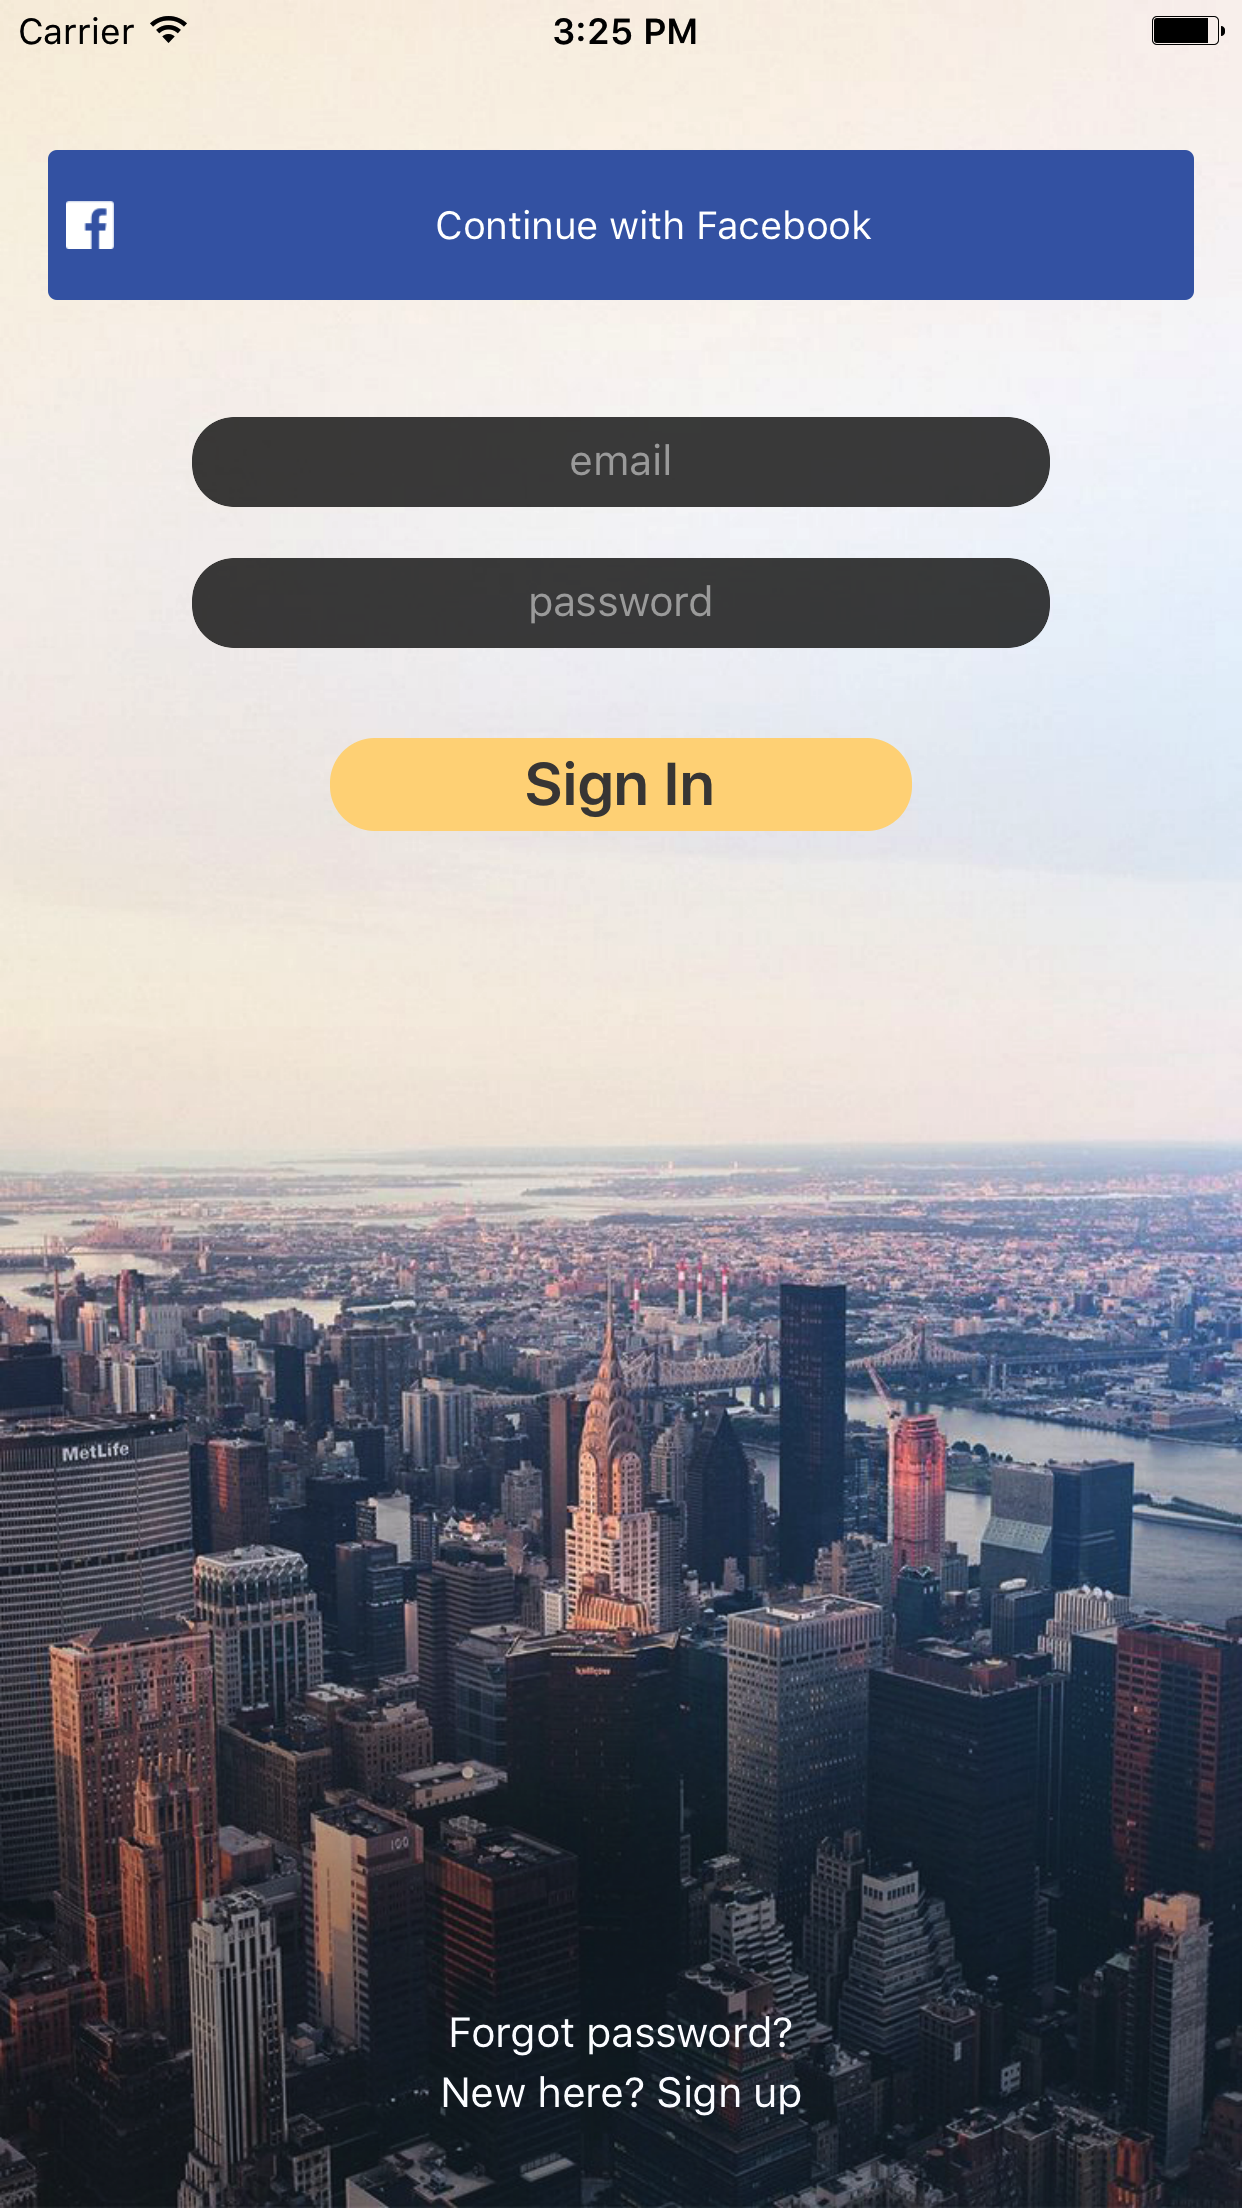
\includegraphics[scale=0.3]{login}
        \end{center}
    \end{column}
    \begin{column}{0.3\textwidth}  %%<--- here
        \begin{center}
            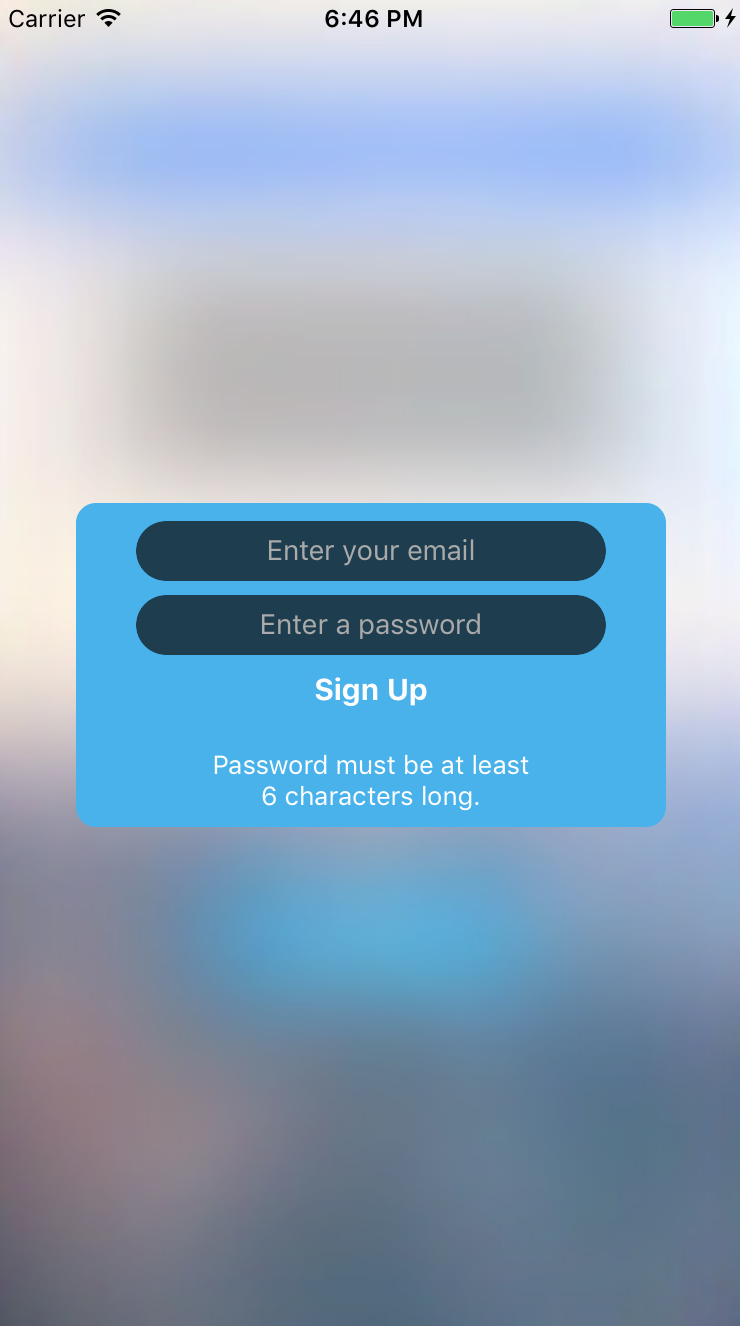
\includegraphics[scale=0.3]{registration}
        \end{center}
    \end{column}
\end{columns}
\end{frame}

\section{Settings}
\begin{frame}
\frametitle{Settings}
\begin{columns}
    \begin{column}{0.3\textwidth}
        Settings View
        \begin{itemize}
            \item background \& time format switching
            \item logout
            \item delete account
        \end{itemize}
    \end{column}
    \begin{column}{0.3\textwidth}  %%<--- here
        \begin{center}
            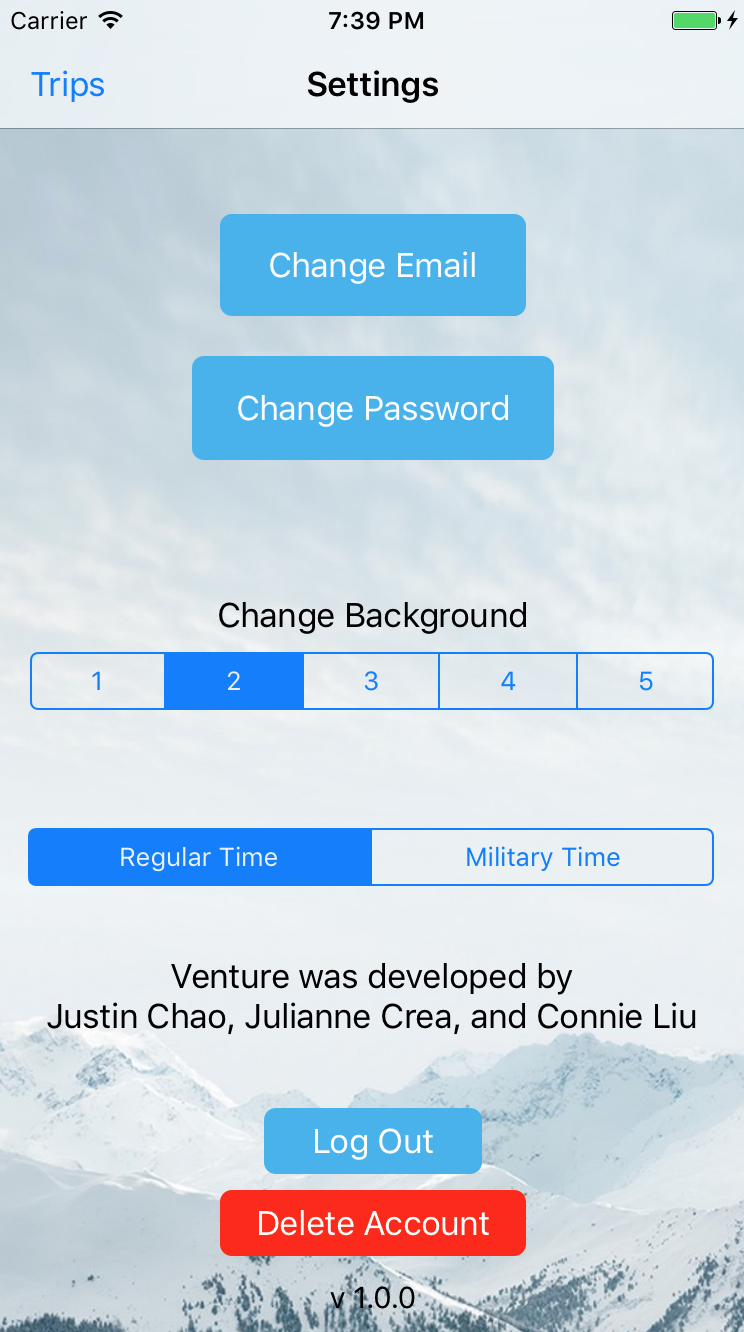
\includegraphics[scale=0.3]{settings}
        \end{center}
    \end{column}
    \begin{column}{0.3\textwidth}  %%<--- here
        \begin{center}
            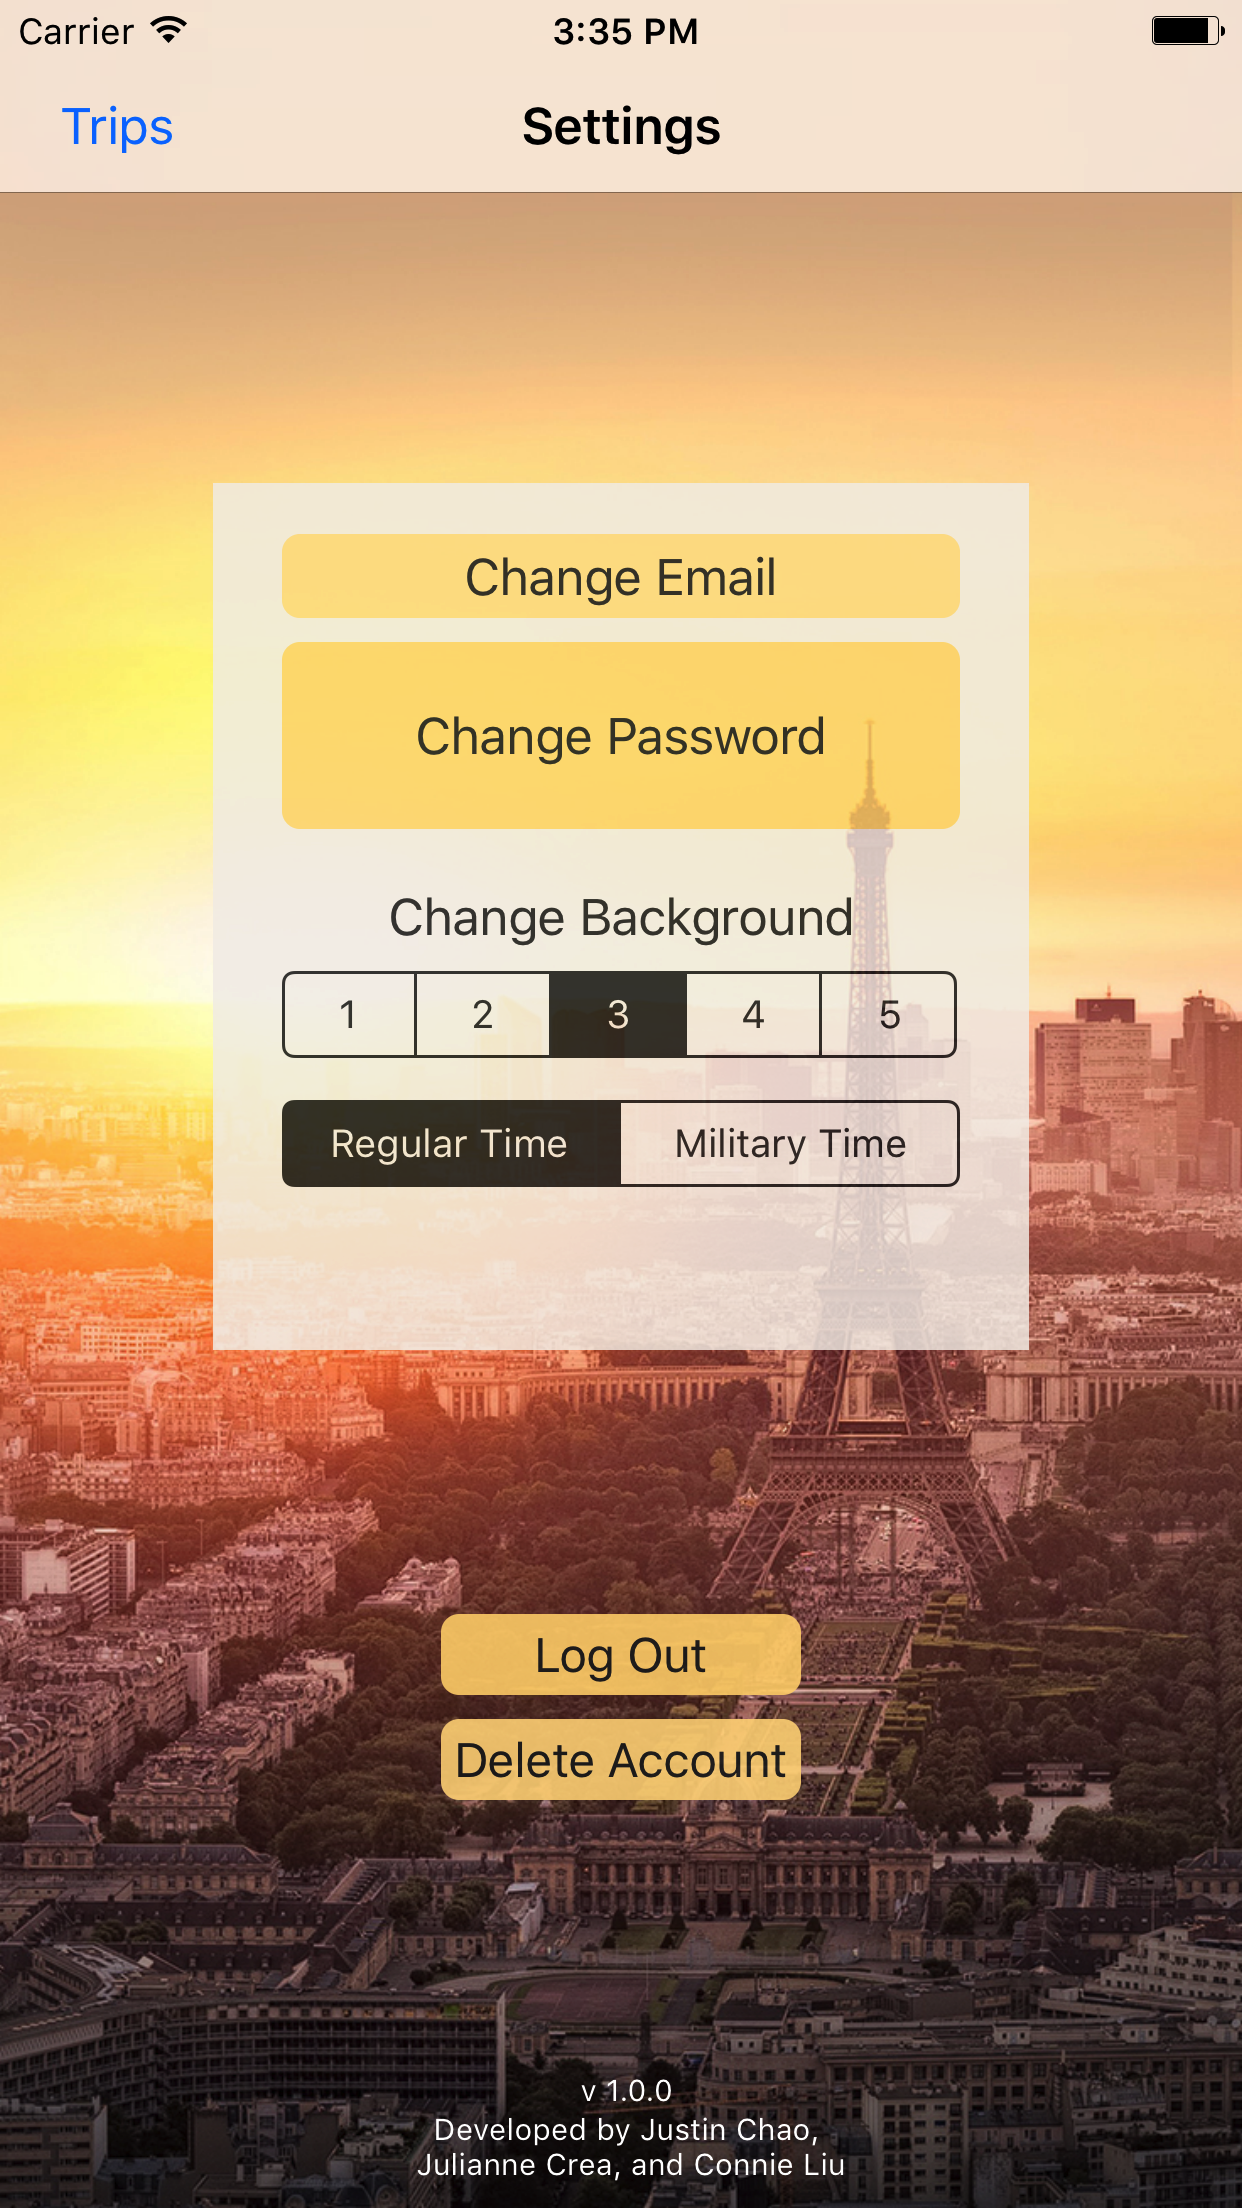
\includegraphics[scale=0.3]{settings2}
        \end{center}
    \end{column}
\end{columns}
\end{frame}

\section{Trips}
\begin{frame}
\frametitle{Trips}
\begin{columns}
    \begin{column}{0.3\textwidth}
        Trips View
        \begin{itemize}
            \item Trip Creation
            \item Your Trips
        \end{itemize}
    \end{column}
    \begin{column}{0.3\textwidth}  %%<--- here
        \begin{center}
            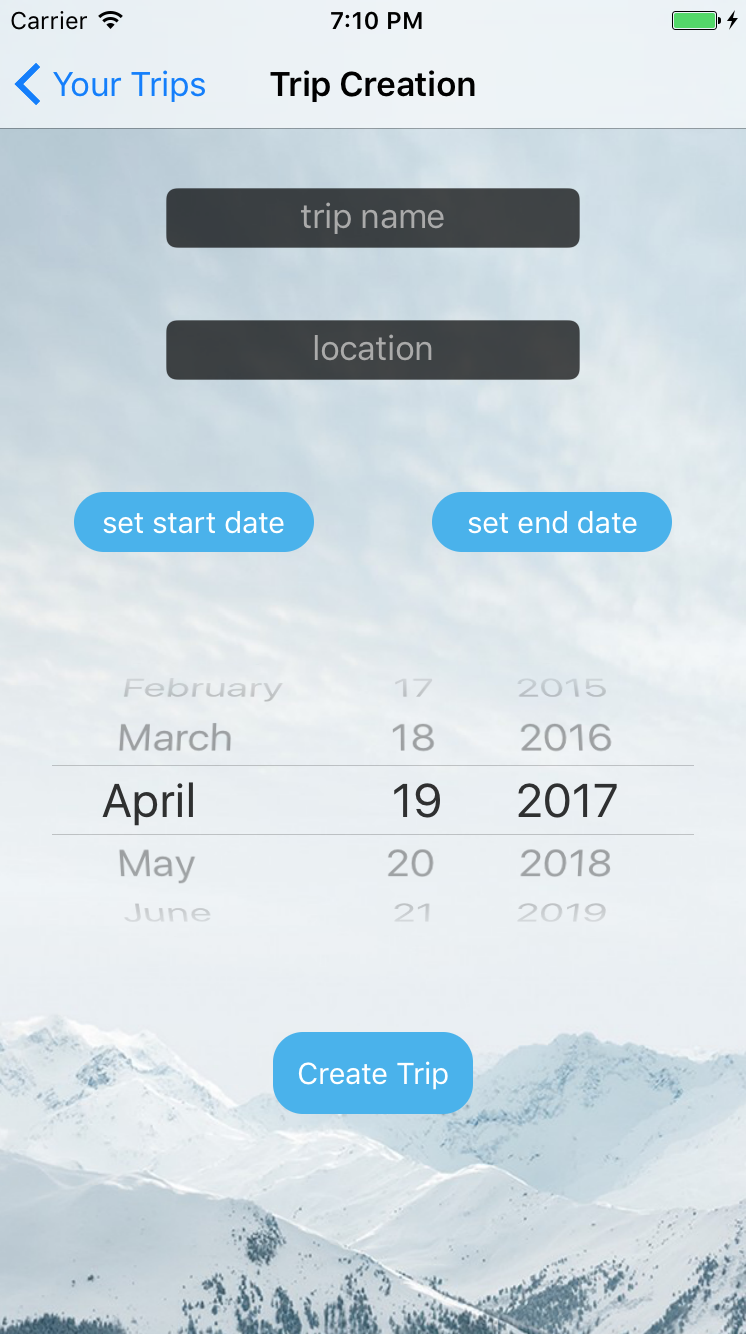
\includegraphics[scale=0.3]{newTrip}
        \end{center}
    \end{column}
    \begin{column}{0.3\textwidth}  %%<--- here
        \begin{center}
            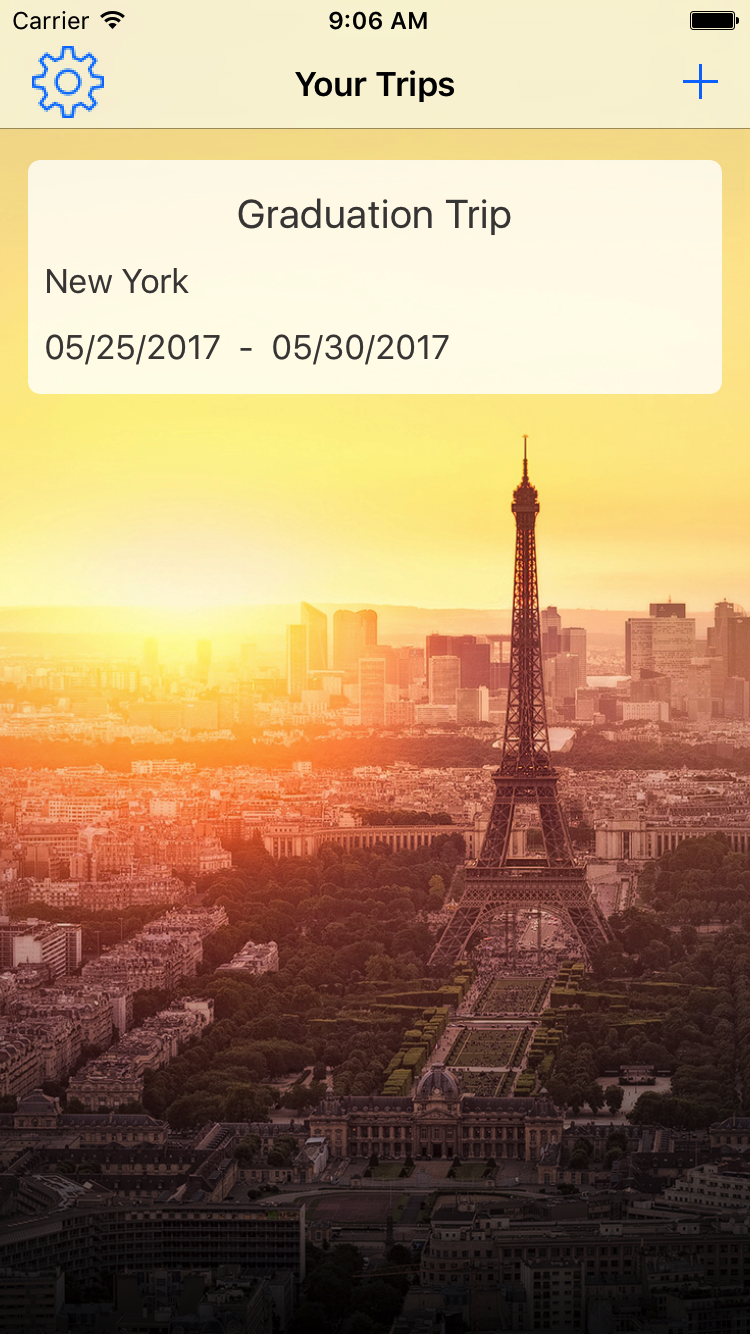
\includegraphics[scale=0.3]{trips}
        \end{center}
    \end{column}
\end{columns}
\end{frame}

\section{Itinerary}
\begin{frame}
\frametitle{Itinerary}
\begin{columns}
    \begin{column}{0.3\textwidth}
        Itinerary View
        \begin{itemize}
            \item itinerary views
        \end{itemize}
    \end{column}
    \begin{column}{0.3\textwidth}  %%<--- here
        \begin{center}
            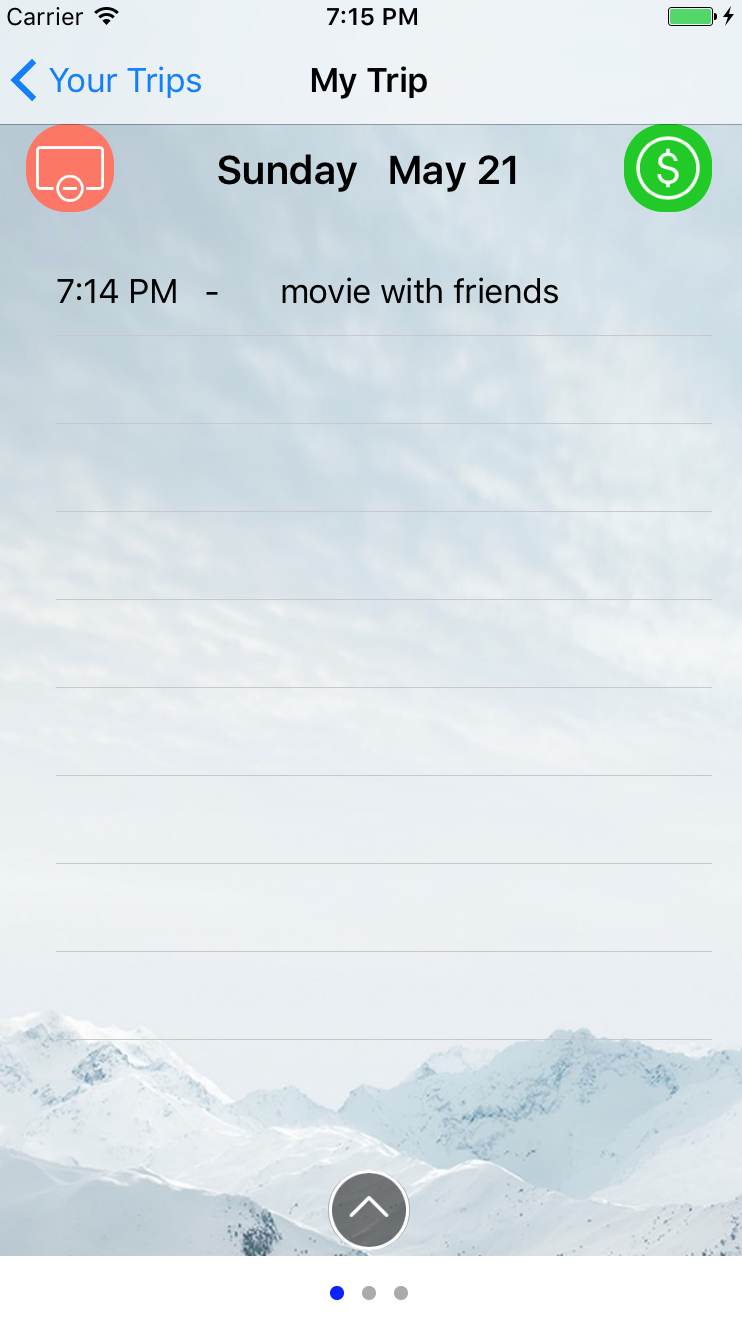
\includegraphics[scale=0.3]{itinerary}
        \end{center}
    \end{column}
    \begin{column}{0.3\textwidth}  %%<--- here
        \begin{center}
            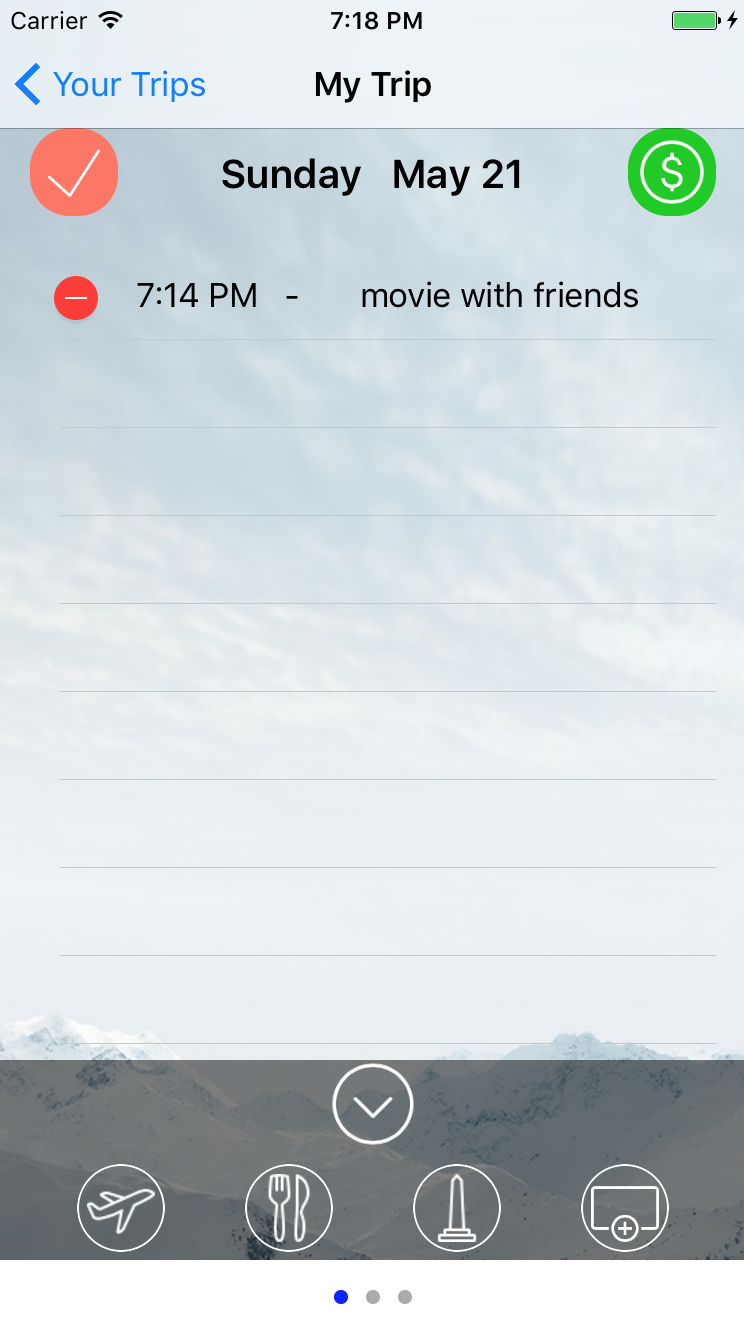
\includegraphics[scale=0.3]{itinerary2}
        \end{center}
    \end{column}
\end{columns}
\end{frame}

\section{Event/Budget}
\begin{frame}
\frametitle{Add Event/Budget}
\begin{columns}
    \begin{column}{0.3\textwidth}
        \begin{itemize}
            \item Event Creation
            \item Budget View
        \end{itemize}
    \end{column}
    \begin{column}{0.3\textwidth}  %%<--- here
        \begin{center}
            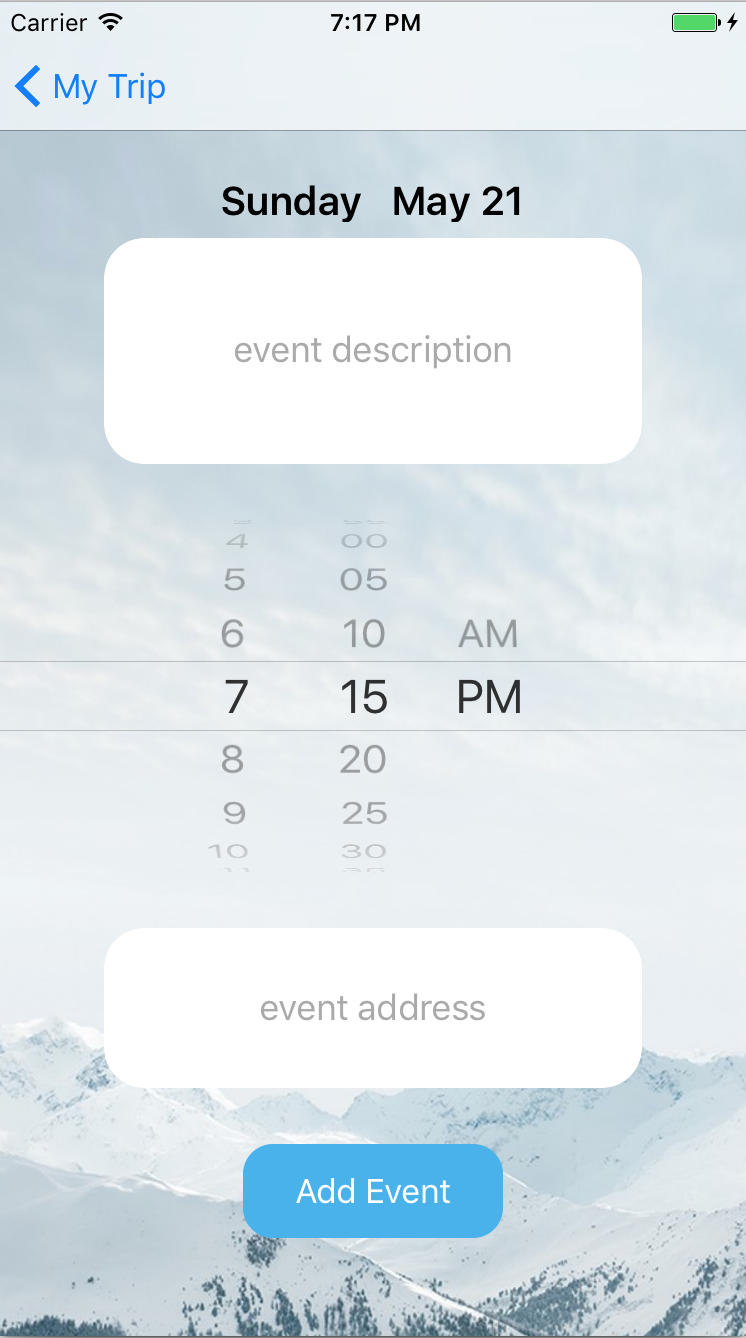
\includegraphics[scale=0.3]{addEvent}
        \end{center}
    \end{column}
    \begin{column}{0.3\textwidth}  %%<--- here
        \begin{center}
            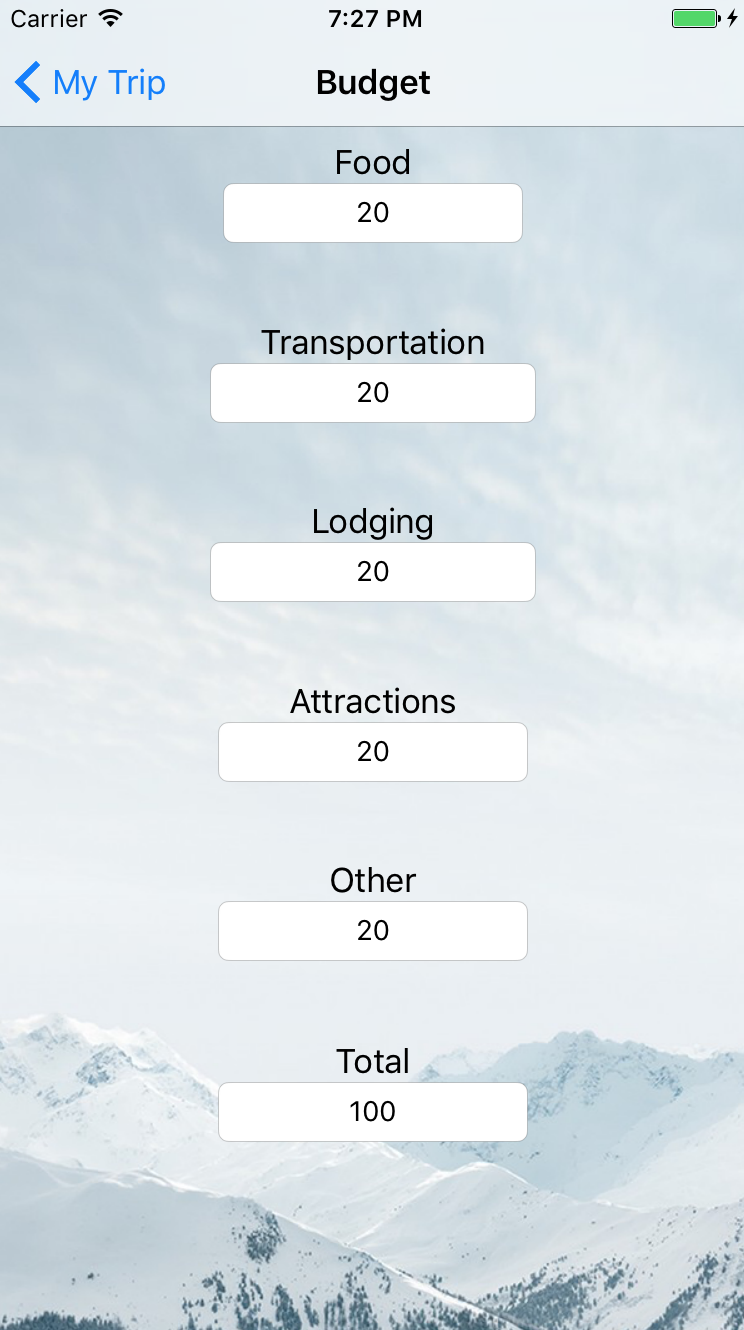
\includegraphics[scale=0.3]{budget}
        \end{center}
    \end{column}
\end{columns}
\end{frame}

\section{Food}
\begin{frame}
\frametitle{Food}
\begin{columns}
    \begin{column}{0.3\textwidth}
        \begin{center}
            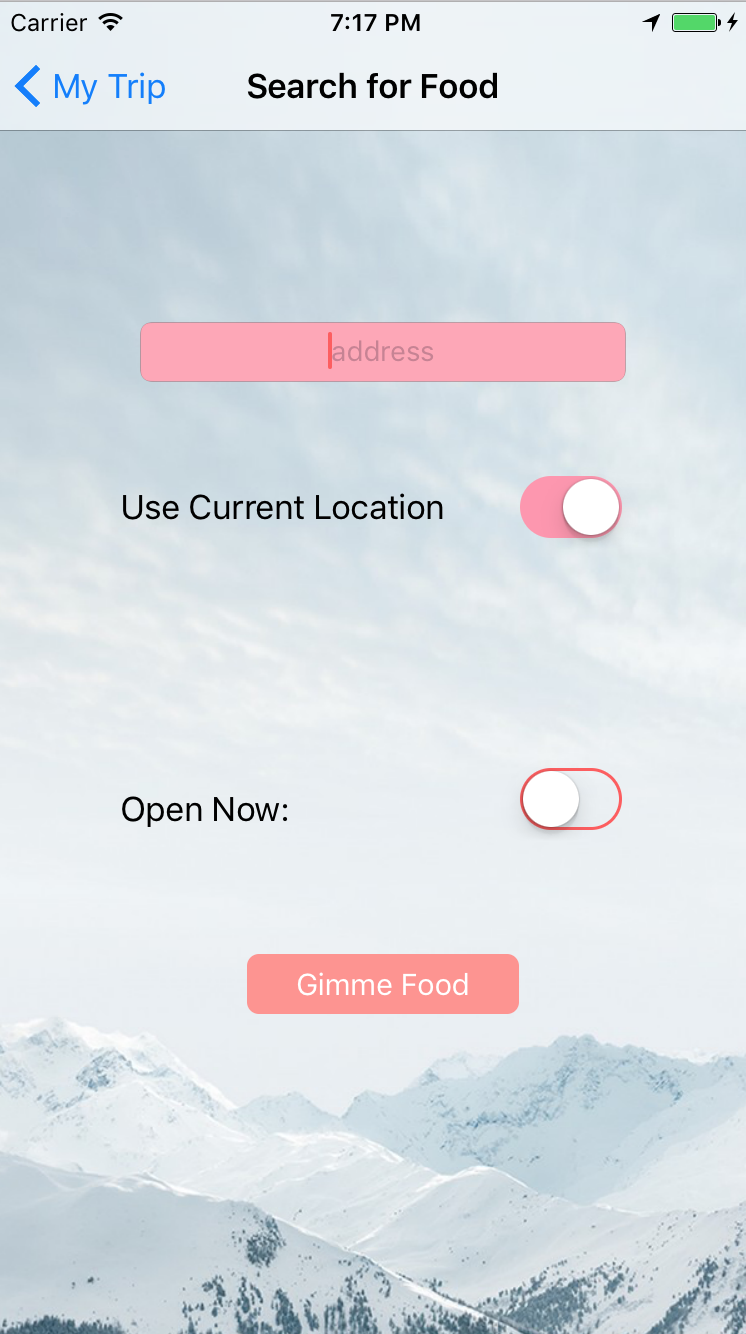
\includegraphics[scale=0.3]{foodSearch}
        \end{center}
    \end{column}
    \begin{column}{0.3\textwidth}  %%<--- here
        \begin{center}
            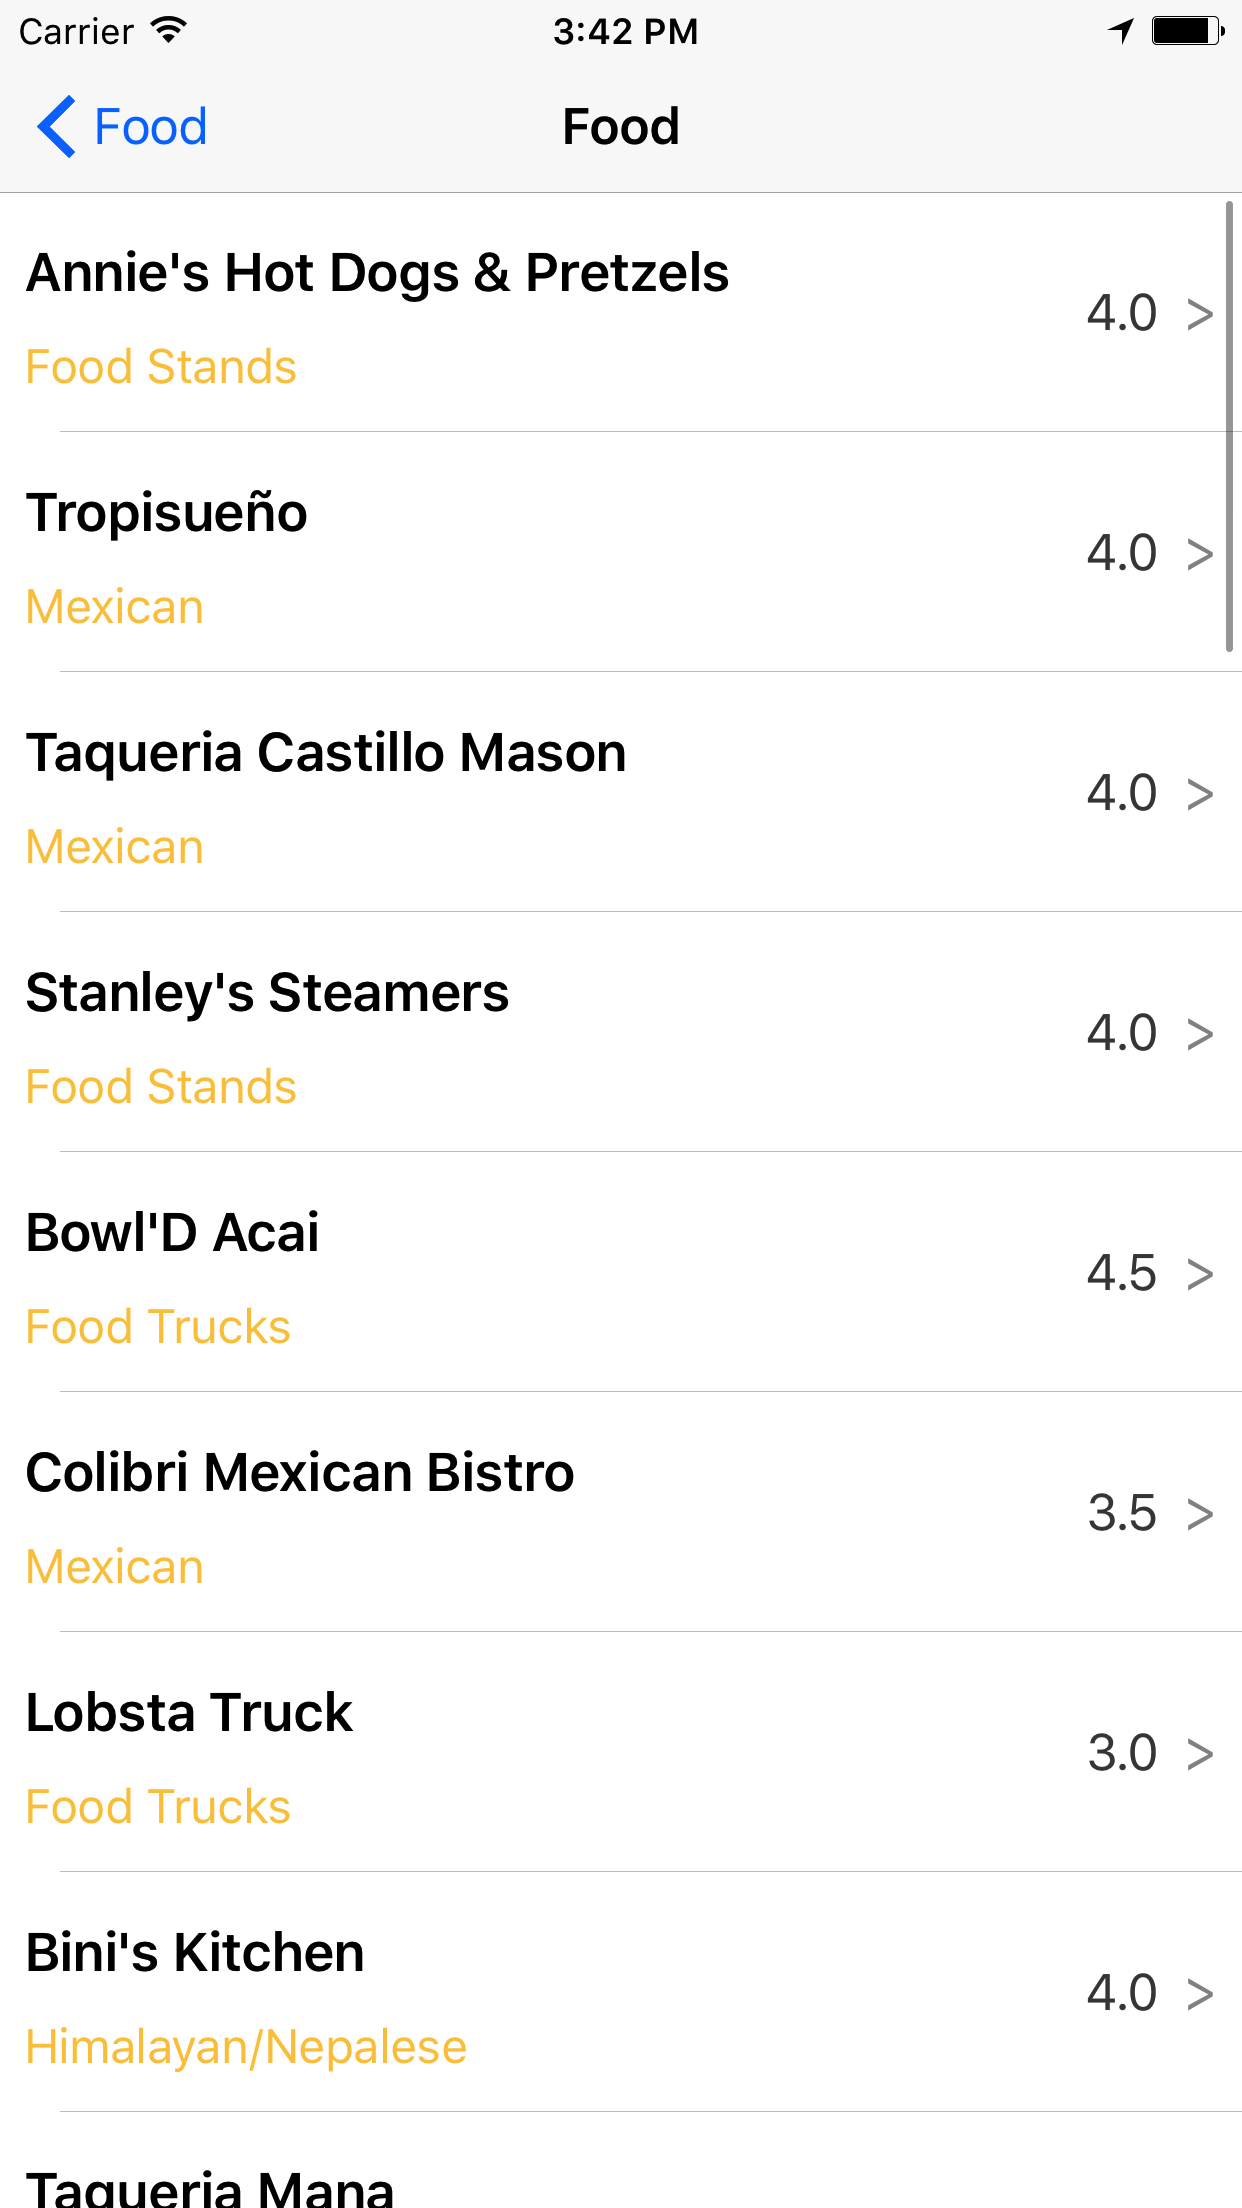
\includegraphics[scale=0.3]{foodTable}
        \end{center}
    \end{column}
    \begin{column}{0.3\textwidth}  %%<--- here
        \begin{center}
            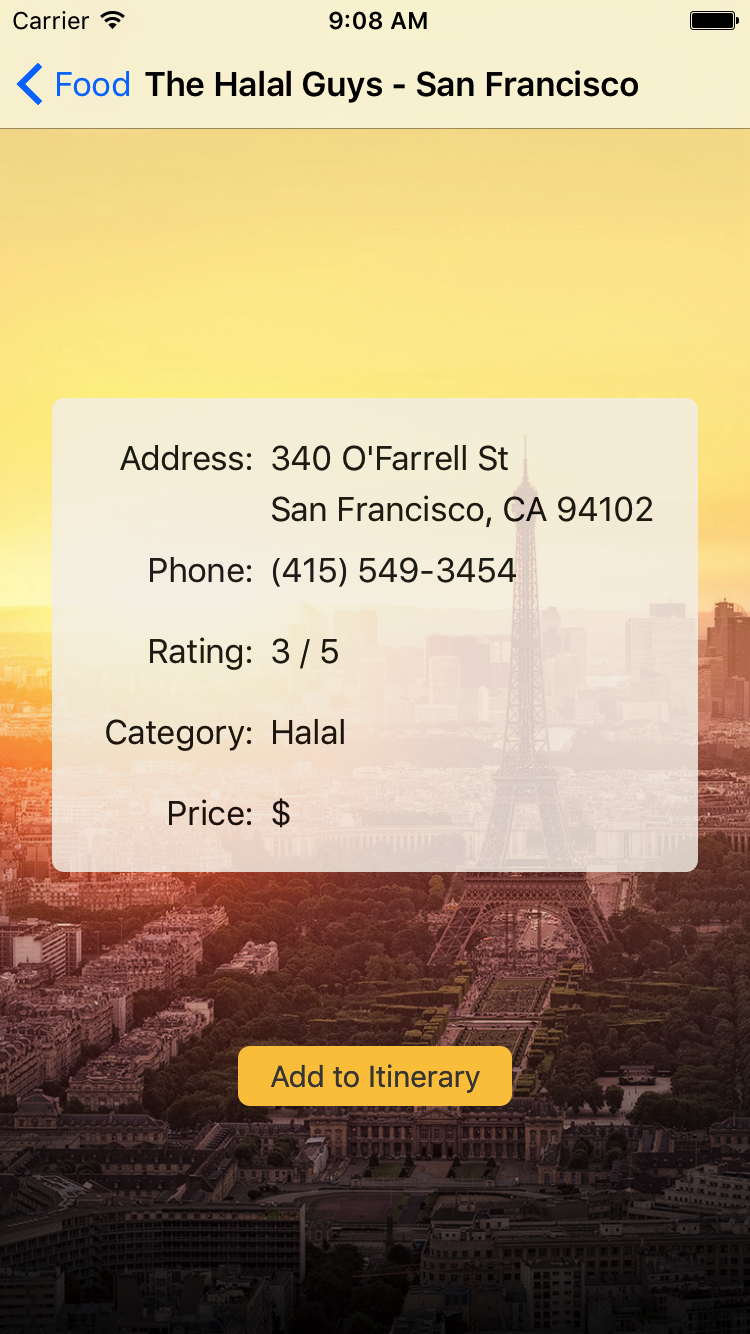
\includegraphics[scale=0.3]{foodDetail}
        \end{center}
    \end{column}
\end{columns}
\end{frame}

\section{Places}
\begin{frame}
\frametitle{Places}
\begin{columns}
    \begin{column}{0.3\textwidth}
        \begin{center}
            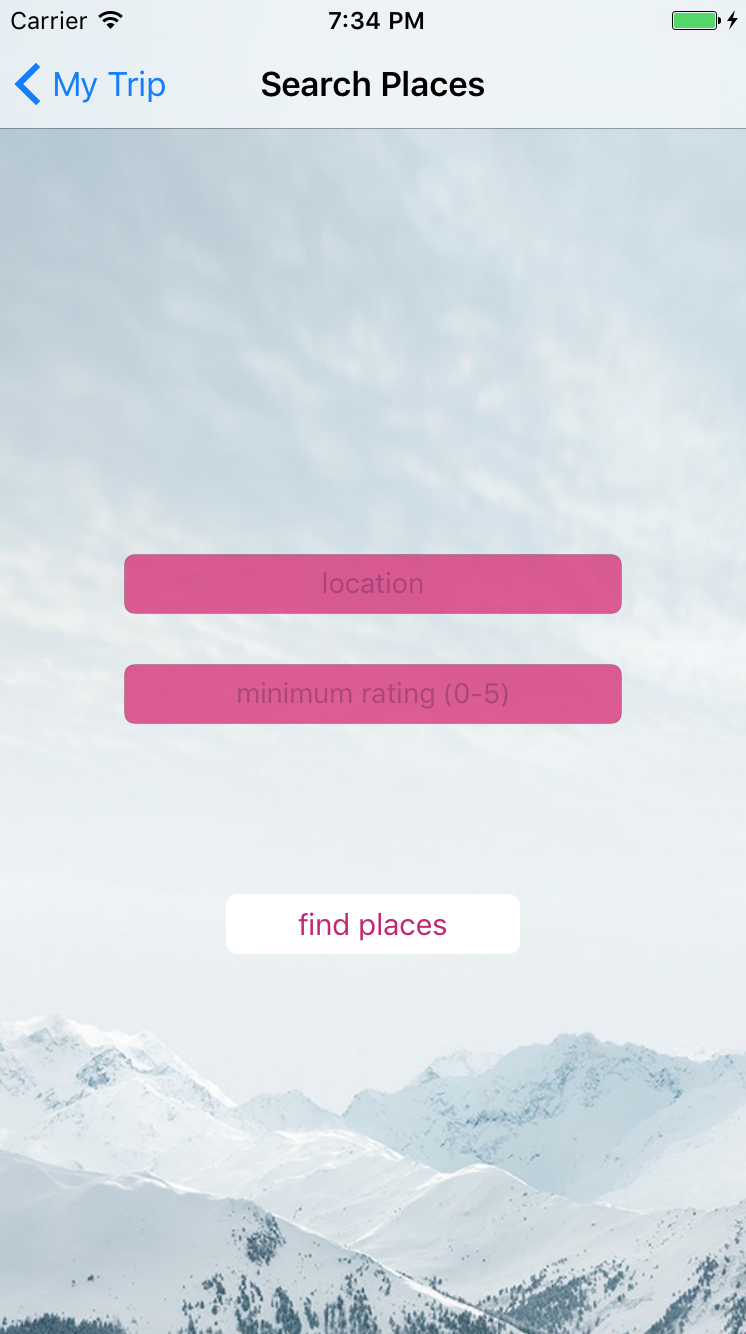
\includegraphics[scale=0.3]{placeSearch}
        \end{center}
    \end{column}
    \begin{column}{0.3\textwidth}  %%<--- here
        \begin{center}
            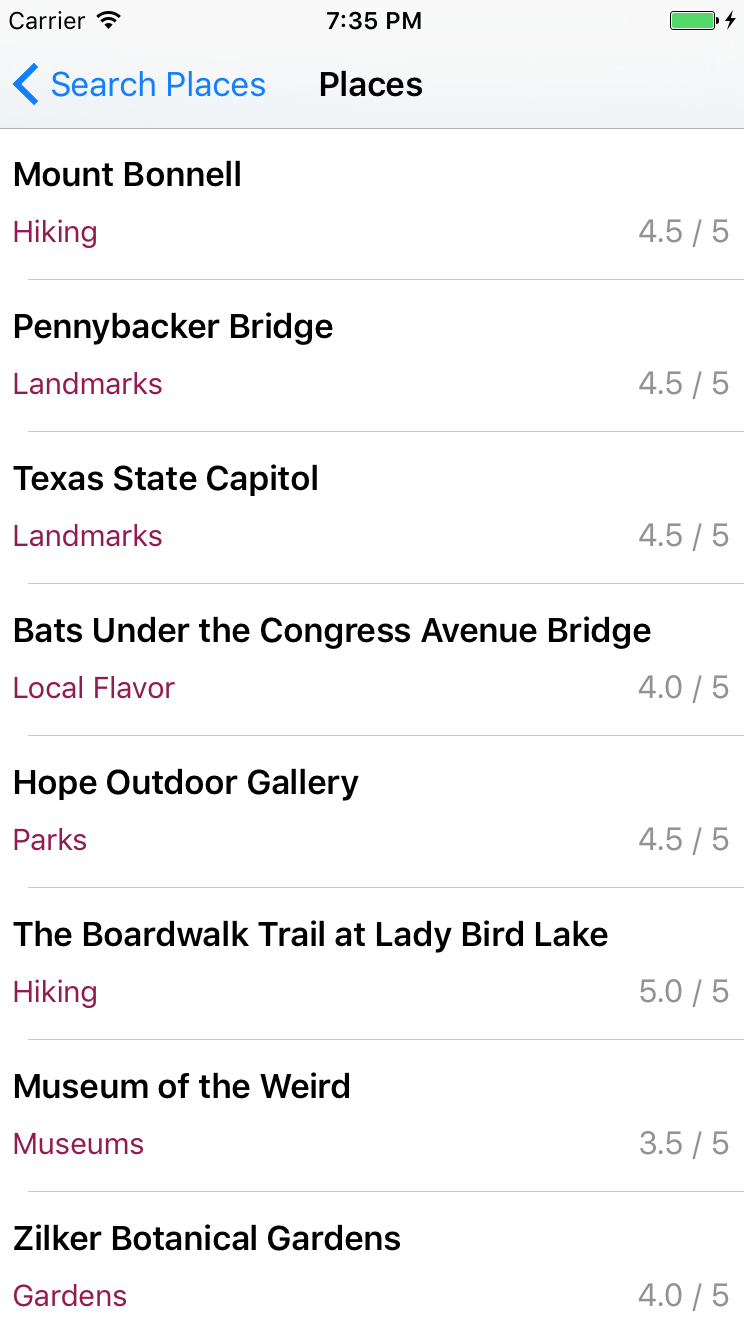
\includegraphics[scale=0.3]{placeTable}
        \end{center}
    \end{column}
    \begin{column}{0.3\textwidth}  %%<--- here
        \begin{center}
            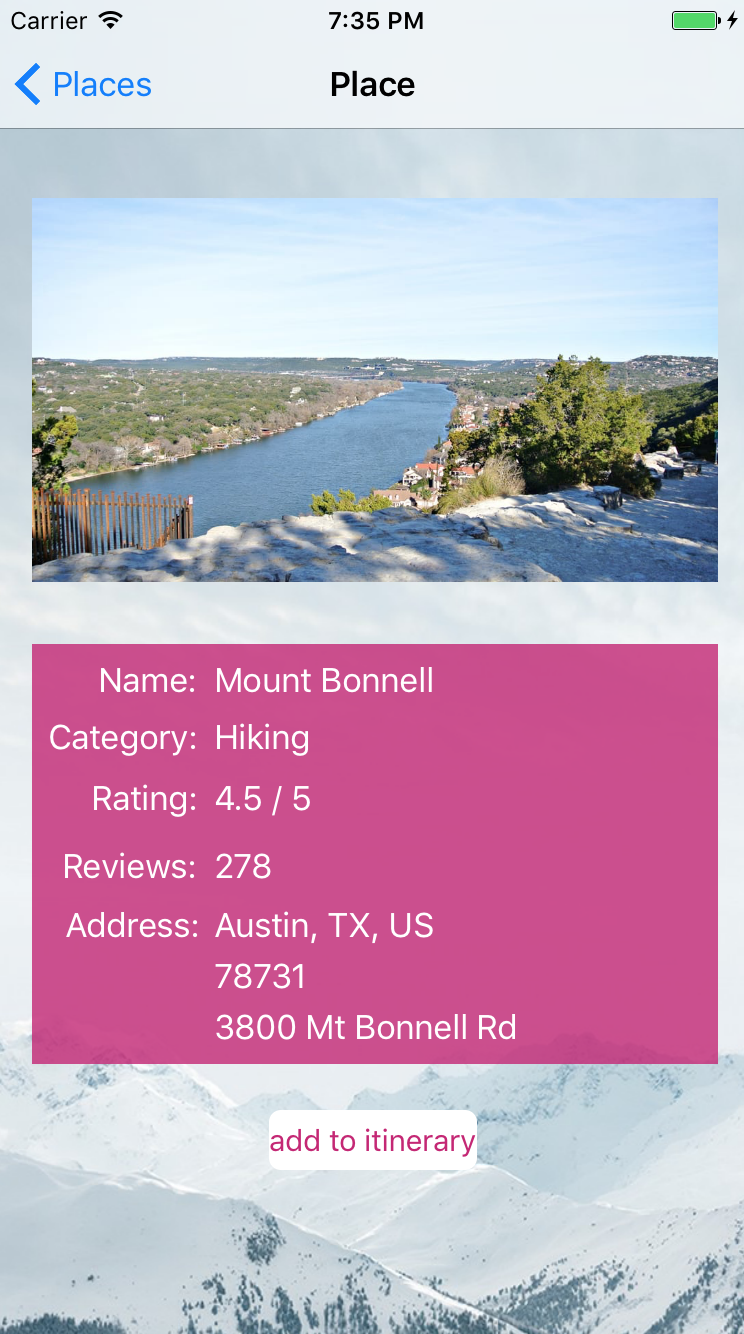
\includegraphics[scale=0.3]{placeDetail}
        \end{center}
    \end{column}
\end{columns}
\end{frame}

\section{Flights}
\begin{frame}
\frametitle{Flights}
\begin{columns}
    \begin{column}{0.3\textwidth}
        \begin{center}
            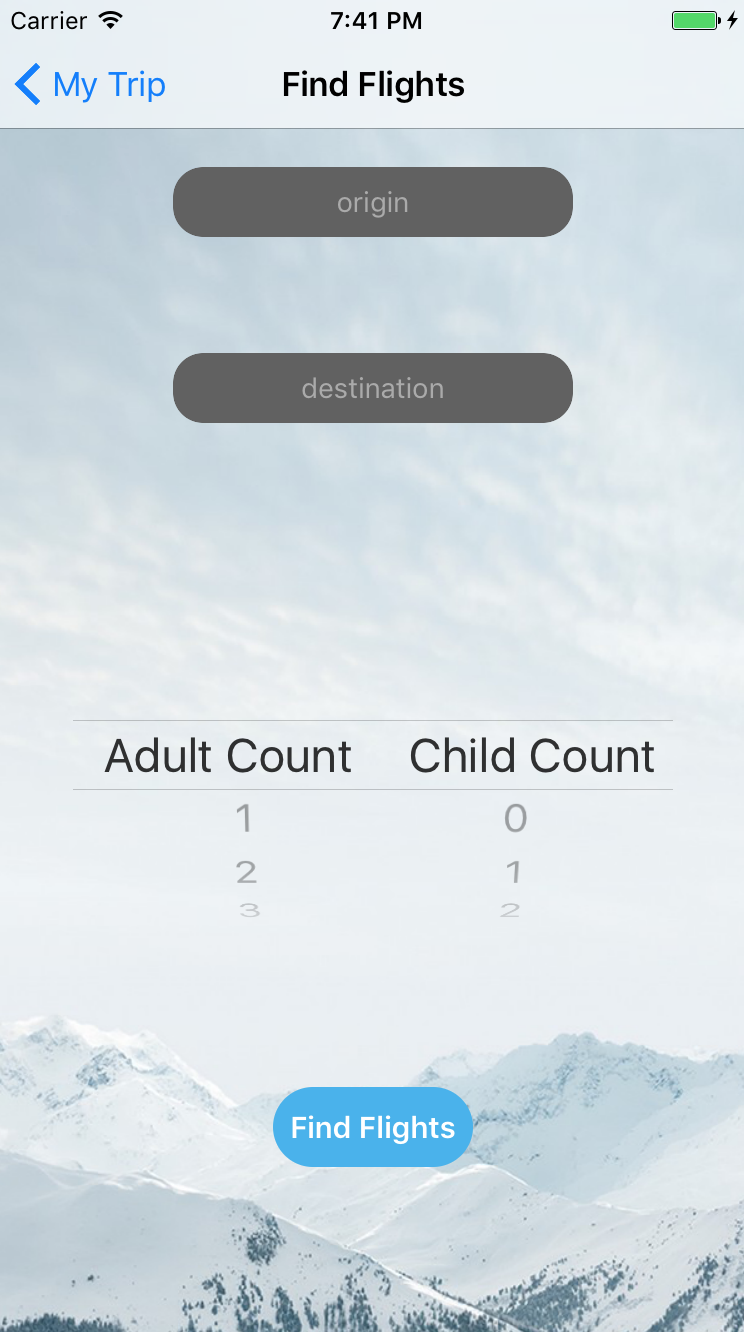
\includegraphics[scale=0.3]{flightSearch}
        \end{center}
    \end{column}
    \begin{column}{0.3\textwidth}  %%<--- here
        \begin{center}
            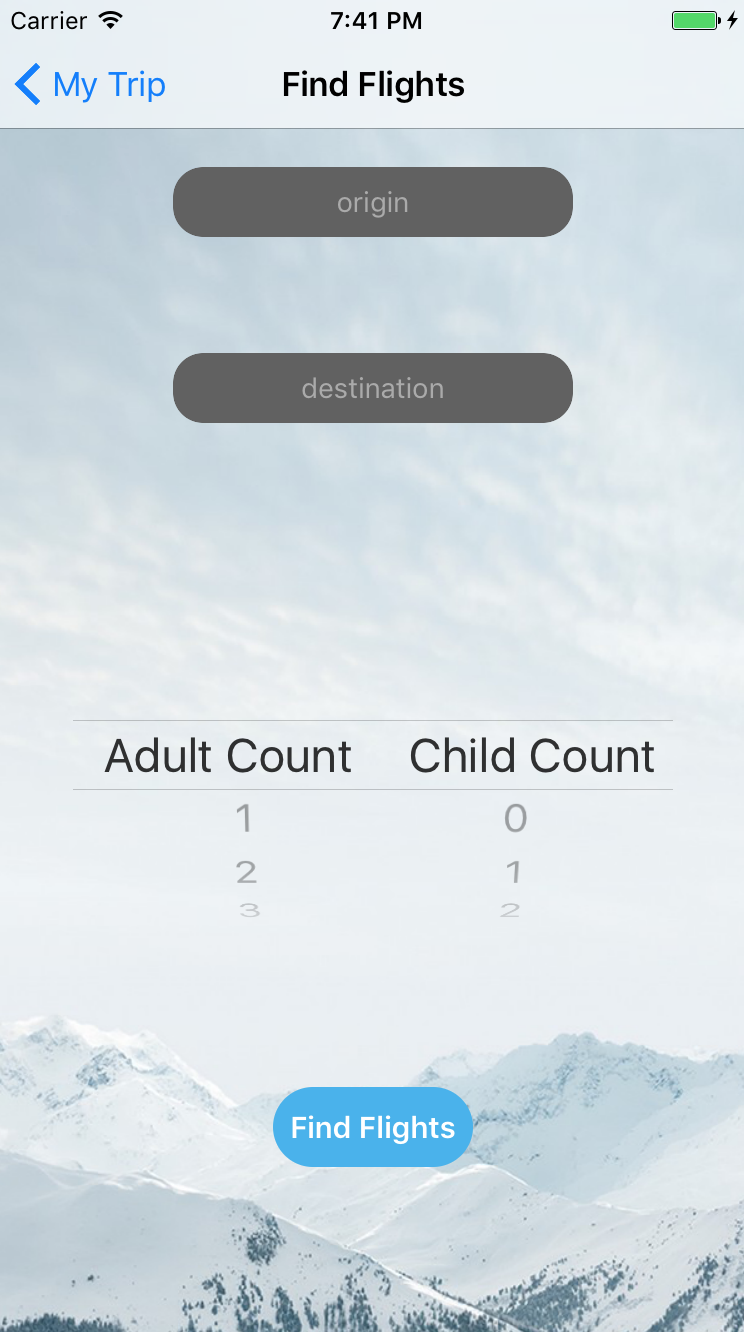
\includegraphics[scale=0.3]{flightSearch}
        \end{center}
    \end{column}
    \begin{column}{0.3\textwidth}  %%<--- here
        \begin{center}
            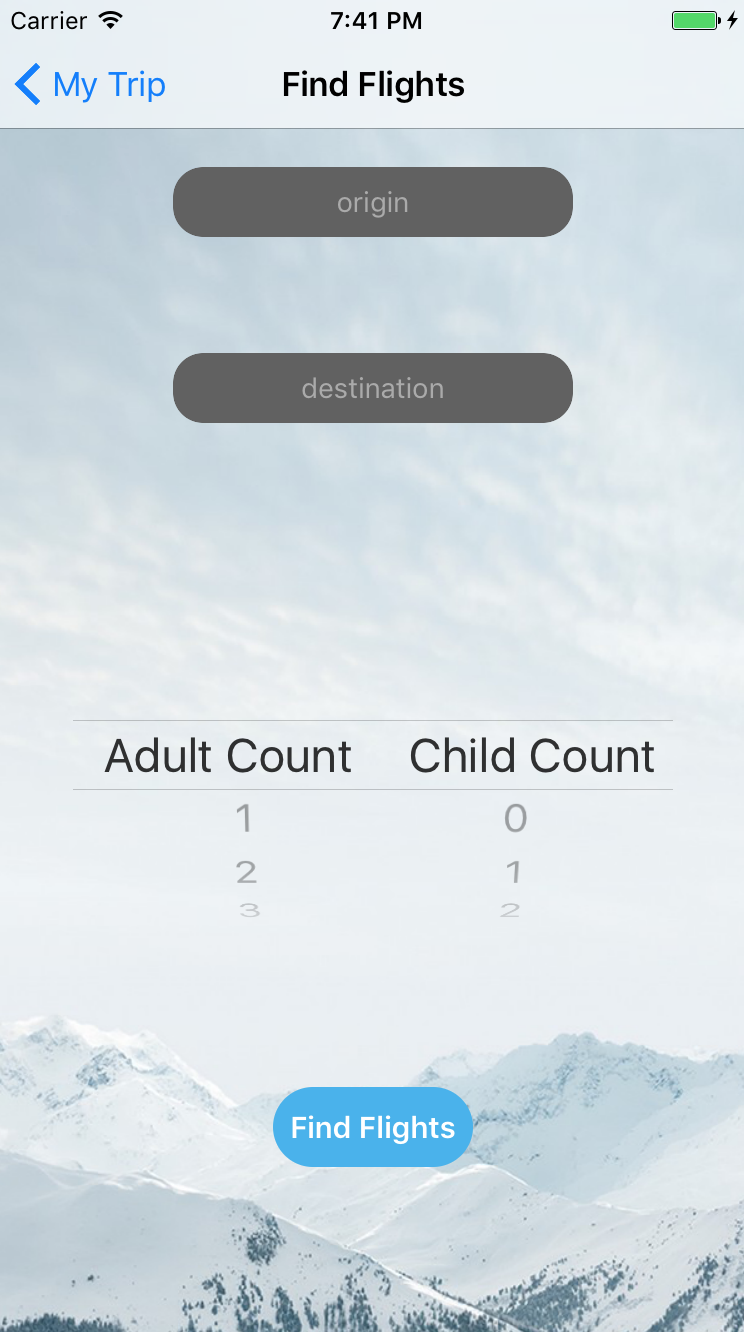
\includegraphics[scale=0.3]{flightSearch}
        \end{center}
    \end{column}
\end{columns}
\end{frame}

\section{Demo}
\begin{frame}
\frametitle{Demo}
    \begin{center}
        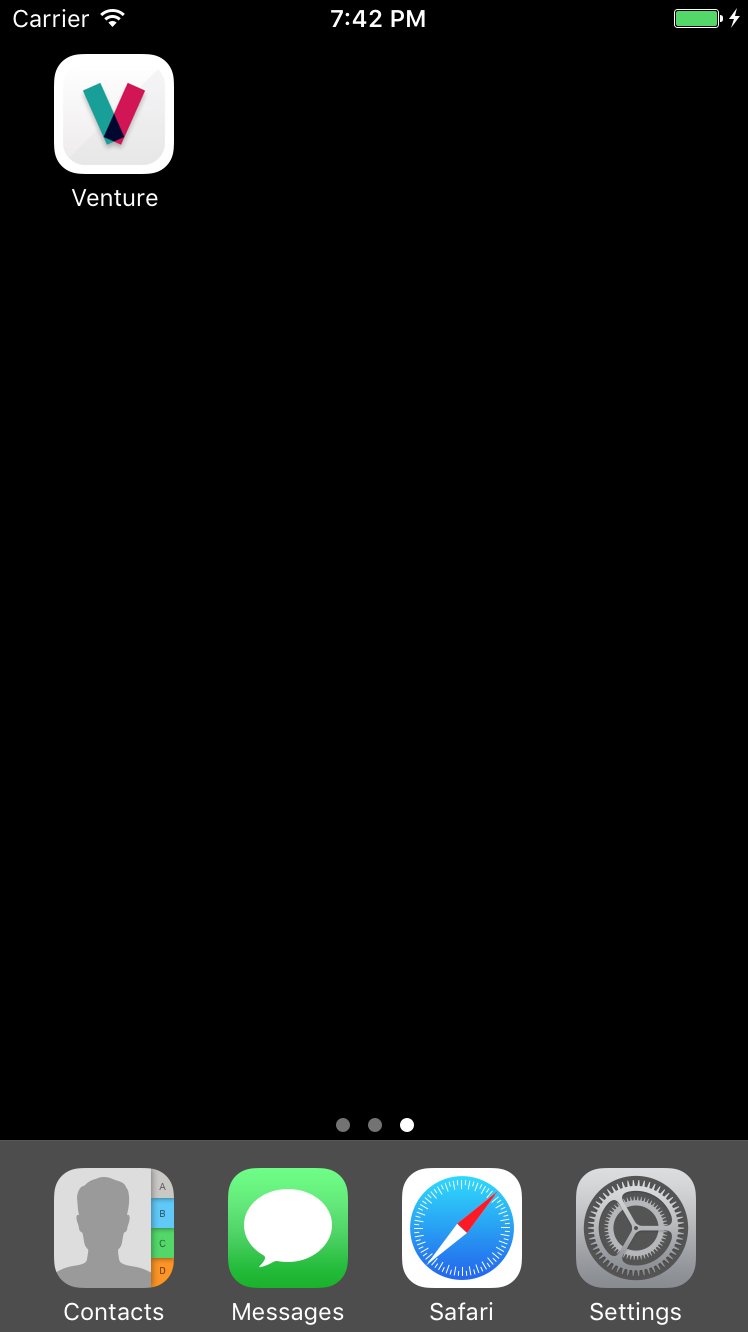
\includegraphics[scale=0.3]{home}
    \end{center}
\end{frame}

\section{Questions \& Answers}
\begin{frame}
\frametitle{Questions \& Answers}
\end{frame}

\end{document}
